\documentclass{article}

% NeurIPS 2026 style — preprint mode shows author names
\usepackage[preprint]{neurips_2026}

\usepackage[utf8]{inputenc}
\usepackage[T1]{fontenc}
\usepackage{hyperref}
\usepackage{url}
\usepackage{booktabs}
\usepackage{amsfonts}
\usepackage{amsmath}
\usepackage{nicefrac}
\usepackage{microtype}
\usepackage{xcolor}
\usepackage{graphicx}
\usepackage{multirow}
\usepackage{algorithm}
\usepackage{algorithmicx}
\usepackage{algpseudocode}
\usepackage{tikz}
\usetikzlibrary{shapes.geometric, arrows.meta, positioning, fit, backgrounds, calc}

% ── Helpful macros ─────────────────────────────────────────────────────────────
\newcommand{\system}{\textsc{CascadeRoute}}
\newcommand{\smallmdl}{GPT-4o-mini}
\newcommand{\largemdl}{GPT-4o}
\definecolor{layer0col}{HTML}{2C3E50}
\definecolor{layer1col}{HTML}{1A5276}
\definecolor{layer2col}{HTML}{1F618D}
\definecolor{smallcol}{HTML}{27AE60}
\definecolor{largecol}{HTML}{E74C3C}

% ── Title & Author ─────────────────────────────────────────────────────────────
\title{Three-Layer Cascaded Routing for Cost-Efficient\\
and Personalized Large Language Model Serving}

\author{%
  Sandeep Vijayarao \\
  Khoury College of Computer Sciences \\
  Northeastern University \\
  Boston, MA 02115 \\
  \texttt{vijayarao.s@northeastern.edu}
}

\begin{document}

\maketitle

% ══════════════════════════════════════════════════════════════════════════════
\begin{abstract}
Serving user queries with large language models (LLMs) is expensive when every
request is unconditionally forwarded to the most capable—and most
costly—model available. We present \system{}, a production-style dual-LLM
serving architecture that routes each query through a three-layer decision
cascade: (1) a word-count pre-flight check, (2) a zero-latency ML router
built on TF-IDF with 16 hand-crafted feature tags and logistic regression,
and (3) a LLM-based fallback classifier invoked only when the ML router
is uncertain. Evaluated on 1,500 synthetically labelled queries spanning
21 intent categories, the ML router alone handles \textbf{85.3\%} of
queries with \textbf{92.6\%} routing accuracy, reducing the fraction that
require an LLM routing call from 30.8\% to 14.7\%. Beyond routing, the
system maintains per-user SQLite profiles and a sliding-window conversation
buffer, injecting personalization context only when a per-query relevance
signal deems it necessary. Every routing decision is logged, enabling a
retrain-from-real-traffic self-improvement loop. Code and evaluation suites
are released at \url{https://github.com/sandeepvijayarao09/dual-llm-system}.
\end{abstract}

% ══════════════════════════════════════════════════════════════════════════════
\section{Introduction}
\label{sec:introduction}

The rapid adoption of LLM-powered applications has exposed a fundamental
cost asymmetry: state-of-the-art models such as \largemdl{} are roughly
an order of magnitude more expensive per token than compact models such as
\smallmdl{}, yet most serving stacks route every query—including trivial
greetings, arithmetic lookups, and one-word factual questions—to the
frontier model \citep{chen2023frugalgpt}. Conversely, always routing to
the cheaper model sacrifices quality on queries that genuinely require deep
reasoning, multi-step analysis, or synthesis across domain knowledge.

Optimal serving requires matching query complexity to model capacity at
query time, ideally without incurring an additional LLM inference
call to make the routing decision. Prior work has addressed this through
mixture-of-experts architectures \citep{shazeer2017moe,jiang2024mixtral},
LLM-based routing with learned preferences \citep{ong2024routellm}, and
cascade-style model selection \citep{chen2023frugalgpt}. However, these
approaches either operate at training time, require human preference data,
or use another LLM call for routing—each adding latency or cost.

\textbf{This paper makes four contributions:}
\begin{enumerate}
    \item A \textbf{three-layer routing cascade} (pre-flight $\rightarrow$
          ML router $\rightarrow$ LLM fallback) that routes 85.3\% of
          queries at zero API cost, with the LLM fallback triggered only
          when the ML router's confidence is below a tuned threshold
          ($\tau_\text{ml} = 0.65$).
    \item A \textbf{feature-augmented TF-IDF router} that extends
          bag-of-words representations with 16 hand-crafted binary tags
          encoding linguistic signals (reasoning keywords, code presence,
          question multiplicity, query length) that are highly predictive
          of routing class but sparse in raw text.
    \item A \textbf{conditional personalization mechanism} where user
          profile context is injected into queries only when a per-query
          relevance signal warrants it, avoiding irrelevant or
          privacy-exposing profile leakage on impersonal queries.
    \item A \textbf{self-improving routing loop}: every routing event is
          logged to a SQLite database; high-confidence labels can be
          exported and used to retrain the ML router on real traffic,
          closing the improvement loop without human annotation.
\end{enumerate}

\system{} is evaluated on a 1,500-case synthetic benchmark spanning 21
intent categories, achieving 92.6\% routing accuracy with a 14.7\% LLM
cascade rate—a 4.4 percentage-point improvement in accuracy and 16.1
percentage-point reduction in cascade rate over the baseline
(280-example training set, logistic regression with unigram TF-IDF).

% ══════════════════════════════════════════════════════════════════════════════
\section{Related Work}
\label{sec:related}

\paragraph{LLM Routing and Cascading.}
FrugalGPT \citep{chen2023frugalgpt} formalizes LLM cascading as a
cost-quality optimization problem and shows that routing to cheaper models
first—escalating only on low-confidence outputs—reduces costs by up to
98\% at matched quality. RouteLLM \citep{ong2024routellm} learns a router
from human preference data (e.g., Chatbot Arena judgements), achieving
strong routing accuracy without LLM calls at inference time. Our work
differs in that we do not require preference labels; instead, we use a
hand-labelled intent taxonomy and hand-crafted features that encode
domain knowledge about query complexity, enabling cold-start routing with
small training sets.

\paragraph{Mixture of Experts.}
Sparse mixture-of-experts (MoE) architectures \citep{shazeer2017moe}
route tokens to specialized sub-networks at every layer of a neural
network. Mixtral \citep{jiang2024mixtral} scales this to frontier LLMs.
These approaches route \emph{within} a model at training time, while our
system routes \emph{between} independently deployed models at serving time,
making it applicable to API-only deployment scenarios.

\paragraph{LLM Blending and Orchestration.}
LLM-Blender \citep{jiang2023llmblender} ensembles outputs from multiple
LLMs through ranking and fusion. HuggingGPT \citep{shen2023hugginggpt}
uses an LLM as an orchestrator to call specialized models as tools. Our
work is complementary: \system{} focuses on efficient routing \emph{before}
inference (not post-hoc blending or tool selection).

\paragraph{Personalization in NLP.}
Prior work on personalized language generation has used user embeddings
\citep{li2023personalized} or retrieval-augmented approaches to condition
model outputs on user history. \system{} takes a simpler, systems-level
approach: embedding structured profile fields directly in the user message,
conditioned on a per-query relevance flag, rather than training personalized
model weights.

% ══════════════════════════════════════════════════════════════════════════════
\section{System Architecture}
\label{sec:architecture}

Figure~\ref{fig:arch} shows the end-to-end routing pipeline. A user query
enters the system and traverses up to three decision layers before being
dispatched to either the Small LLM (\smallmdl{}) or the Large LLM
(\largemdl{}). The layers are designed in order of increasing cost and
decreasing throughput, ensuring that the cheapest sufficient gate handles
each query.

\begin{figure}[t]
\centering
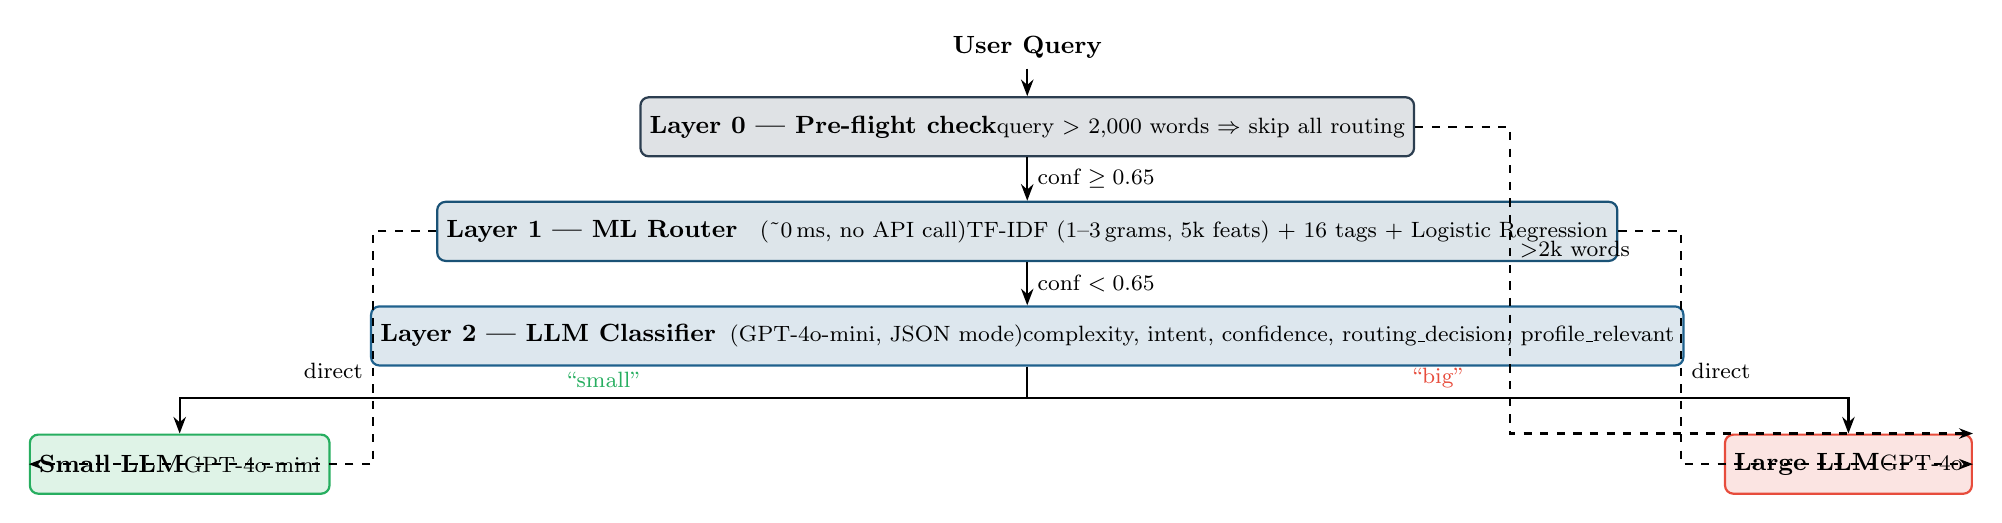
\begin{tikzpicture}[
    node distance=0.55cm and 1.2cm,
    every node/.style={font=\small},
    box/.style={rectangle, rounded corners=3pt, minimum width=5.8cm,
                minimum height=0.75cm, text centered, draw, thick},
    layer0/.style={box, fill=layer0col!15, draw=layer0col},
    layer1/.style={box, fill=layer1col!15, draw=layer1col},
    layer2/.style={box, fill=layer2col!15, draw=layer2col},
    smallbox/.style={box, fill=smallcol!15, draw=smallcol, minimum width=2.5cm},
    largebox/.style={box, fill=largecol!15, draw=largecol, minimum width=2.5cm},
    arr/.style={-{Stealth[length=6pt]}, thick},
    sidarr/.style={-{Stealth[length=5pt]}, thick, dashed},
]

\node[layer0] (preflight) {\textbf{Layer 0 — Pre-flight check}\\
    \footnotesize query $>$ 2{,}000 words $\Rightarrow$ skip all routing};

\node[layer1, below=of preflight] (mlrouter) {\textbf{Layer 1 — ML Router} \hspace{0.2em}
    {\footnotesize(\textasciitilde{}0\,ms, no API call)}\\
    \footnotesize TF-IDF (1–3\,grams, 5k feats) + 16 tags + Logistic Regression};

\node[layer2, below=of mlrouter] (llmcls) {\textbf{Layer 2 — LLM Classifier}
    \hspace{0.2em}{\footnotesize(\smallmdl{}, JSON mode)}\\
    \footnotesize complexity, intent, confidence, routing\_decision, profile\_relevant};

\node[smallbox, below left=0.85cm and 0.5cm of llmcls] (smallllm)
    {\textbf{Small LLM}\\{\footnotesize \smallmdl{}}};

\node[largebox, below right=0.85cm and 0.5cm of llmcls] (largellm)
    {\textbf{Large LLM}\\{\footnotesize \largemdl{}}};

% Arrows
\draw[arr] (preflight) -- node[right, font=\footnotesize]{conf $\geq 0.65$}
    (mlrouter);
\draw[arr] (mlrouter) -- node[right, font=\footnotesize]{conf $< 0.65$}
    (llmcls);

\draw[arr] (llmcls.south) -- ++(0,-0.4) -| node[above, font=\footnotesize, pos=0.25]
    {\textcolor{smallcol}{``small''}} (smallllm.north);
\draw[arr] (llmcls.south) -- ++(0,-0.4) -| node[above, font=\footnotesize, pos=0.25]
    {\textcolor{largecol}{``big''}} (largellm.north);

% ML router direct output
\draw[sidarr] (mlrouter.west) -- ++(-0.8,0) |- node[left, font=\footnotesize, pos=0.3]
    {direct} (smallllm.west);
\draw[sidarr] (mlrouter.east) -- ++(0.8,0) |- node[right, font=\footnotesize, pos=0.3]
    {direct} (largellm.east);

% Pre-flight bypass
\draw[sidarr] (preflight.east) -- ++(1.2,0) |- node[right, font=\footnotesize, pos=0.2]
    {$>$2k words} (largellm.north east);

% Input arrow
\node[above=0.35cm of preflight, font=\small\bfseries] (query) {User Query};
\draw[arr] (query) -- (preflight);

\end{tikzpicture}
\caption{The \system{} routing pipeline. Solid arrows show the primary path;
dashed arrows show direct routing when the ML router has sufficient confidence
($\geq$\,0.65) or the pre-flight condition fires. The LLM Classifier is only
invoked for $\approx$14.7\% of queries.}
\label{fig:arch}
\end{figure}

\subsection{Layer 0: Pre-flight Check}
\label{sec:layer0}

Queries exceeding 2,000 words are unconditionally dispatched to the Large LLM
without classification. This heuristic handles long documents, code dumps, and
multi-part essays that deterministically require the larger context window and
reasoning budget, and avoids wasting the classifier on degenerate inputs.

\subsection{Layer 1: ML Router}
\label{sec:layer1}

The ML router is a scikit-learn \citep{pedregosa2011sklearn} pipeline
consisting of a TF-IDF vectorizer followed by logistic regression.
Critically, each query is first processed by \texttt{encode\_text()}, which
prepends binary feature tags to the raw query string before vectorization.
This allows the TF-IDF model to attend to tag tokens as first-class features
without requiring a separate feature concatenation step. Full details appear
in Section~\ref{sec:ml_router}.

If the router's predicted class probability exceeds $\tau_\text{ml} = 0.65$,
the routing decision is used directly and no API call is made. Otherwise, the
query cascades to Layer 2.

\subsection{Layer 2: LLM Classifier}
\label{sec:layer2}

The LLM Classifier uses \smallmdl{} in JSON mode to predict six fields:
\texttt{complexity}, \texttt{intent}, \texttt{confidence},
\texttt{requires\_tools}, \texttt{sensitive}, \texttt{routing\_decision},
and \texttt{profile\_relevant}. If the returned confidence is below
$\tau_\text{llm} = 0.75$, or if JSON parsing fails, the system conservatively
defaults to routing \texttt{"big"}. The \texttt{profile\_relevant} flag is
used by the personalization subsystem (Section~\ref{sec:personalization}).

\subsection{Routing Decision Finalization}
\label{sec:finalization}

After the routing layer determines the target model, the orchestrator
applies the profile injection decision and dispatches the query:
\begin{itemize}
    \item \textbf{Small path} (\smallmdl{}, $\leq$512 tokens): the
    \texttt{SimpleAnswerer} module handles the query with optional profile
    augmentation.
    \item \textbf{Large path} (\largemdl{}, $\leq$4096 tokens):
    a three-stage pipeline runs sequentially—(1) \texttt{Reasoner}
    generates the core answer, (2) \texttt{Summarizer} compresses it to
    one sentence using \smallmdl{}, and (3) \texttt{Personalizer} wraps
    the core answer with a personalized introduction and closing using
    \smallmdl{}. The final response is assembled as:
    \texttt{intro + core + "---" + closing}.
\end{itemize}

Algorithm~\ref{alg:routing} formalizes the complete routing procedure.

\begin{algorithm}[t]
\caption{\system{} Query Routing}
\label{alg:routing}
\begin{algorithmic}[1]
\Require query $q$, user profile $P$, user id $\text{uid}$
\Ensure answer $A$, routing metadata $M$
\If{$|\text{words}(q)| > 2000$}
    \State \Return \Call{RouteBig}{$q, P, \text{uid}$}
\EndIf
\State $(y_\text{ml},\, c_\text{ml}) \leftarrow \text{MLRouter.predict}(\text{encode}(q))$
\If{$c_\text{ml} \geq \tau_\text{ml}$} \Comment{$\tau_\text{ml} = 0.65$}
    \State $\text{routing} \leftarrow y_\text{ml}$;\; $\text{routed\_by} \leftarrow \text{"ml"}$
\Else
    \State $\text{cls} \leftarrow \text{LLMClassifier}(q)$ \Comment{JSON mode, \smallmdl{}}
    \State $\text{routing} \leftarrow \text{cls.routing\_decision}$;\; $\text{routed\_by} \leftarrow \text{"llm"}$
\EndIf
\If{$\text{is\_self\_referential}(q)$}
    \State $P_\text{eff} \leftarrow P$ \Comment{full profile always injected}
\ElsIf{$\text{routed\_by} = \text{"llm"}$ \textbf{and} $\text{cls.profile\_relevant}$}
    \State $P_\text{eff} \leftarrow P$
\ElsIf{$\text{routing} = \text{"big"}$}
    \State $P_\text{eff} \leftarrow P$ \Comment{heuristic: complex $\Rightarrow$ relevant}
\Else
    \State $P_\text{eff} \leftarrow \{$\texttt{name}: $P.\text{name}\}$ \Comment{name stub only}
\EndIf
\State \Return \Call{Route}{$q, P_\text{eff}, \text{routing}, \text{uid}$}
\end{algorithmic}
\end{algorithm}

% ══════════════════════════════════════════════════════════════════════════════
\section{ML Router Design}
\label{sec:ml_router}

\subsection{Feature Engineering via Tag Augmentation}
\label{sec:features}

A key challenge for routing is that complexity signals are often sparse in
raw query text—e.g., the word \emph{``why''} strongly predicts a reasoning
query but rarely co-occurs with other complexity markers in short queries,
making TF-IDF alone unreliable. We address this by prepending binary
semantic tags to the query string before vectorization:
\begin{equation}
    \text{encode}(q) = \text{tags}(q) \;\|\; q
\end{equation}
where $\text{tags}(q)$ is a space-separated string of zero or more tokens
from the vocabulary $\mathcal{T}$ described in Table~\ref{tab:features}.

\begin{table}[t]
\caption{Feature tag vocabulary. Each tag fires when its pattern matches
the query and is prepended to the raw query before TF-IDF encoding.
Routing hint indicates the class the tag biases toward.}
\label{tab:features}
\centering
\small
\begin{tabular}{llp{4.8cm}l}
\toprule
\textbf{Tag} & \textbf{Signal} & \textbf{Trigger condition} & \textbf{Hint} \\
\midrule
\texttt{LEN\_SHORT}       & query length & $\leq$8 words        & small \\
\texttt{LEN\_MEDIUM}      & query length & 9--40 words          & neutral \\
\texttt{LEN\_LONG}        & query length & $>$40 words          & big \\
\texttt{HAS\_CODE}        & syntax       & \texttt{```}, \texttt{def}, \texttt{class}, \texttt{import} & big \\
\texttt{HAS\_MATH}        & notation     & digits+operators, \texttt{\textbackslash{}int}, \texttt{\textbackslash{}sum} & big \\
\texttt{HAS\_REASONING\_KW}  & semantics & why, how, compare, prove, explain, analyze & big \\
\texttt{HAS\_FACTUAL\_KW}    & semantics & what is, who is, when did, define & small \\
\texttt{HAS\_GREETING\_KW}   & social    & hi, hello, thanks, bye & small \\
\texttt{HAS\_CREATIVE\_KW}   & task type & joke, poem, story, haiku, pun & small \\
\texttt{HAS\_OPINION\_KW}    & semantics & best, vs, should I, pros and cons & big \\
\texttt{HAS\_DEEP\_WHAT}     & abstraction & ``what is'' + $>$5 words & big \\
\texttt{HAS\_IMPACT\_KW}     & semantics & impact, effect, consequence & big \\
\texttt{HAS\_RESEARCH\_KW}   & domain    & research, literature, studies show & big \\
\texttt{HAS\_SELF\_REF}      & profile   & my name, who am I, about me & inject \\
\texttt{Q\_MULTI}            & structure & $\geq$2 question marks & big \\
\texttt{MULTI\_SENTENCE}     & structure & $\geq$3 sentence-ending punctuation & big \\
\bottomrule
\end{tabular}
\end{table}

The tag vocabulary encodes expert knowledge about query complexity: reasoning
keywords (\texttt{HAS\_REASONING\_KW}), abstract definitions (\texttt{HAS\_DEEP\_WHAT}),
code presence (\texttt{HAS\_CODE}), and compound questions (\texttt{Q\_MULTI}) are strong
predictors of queries that require the Large LLM. Greeting keywords
(\texttt{HAS\_GREETING\_KW}), short queries (\texttt{LEN\_SHORT}), and factual
lookups (\texttt{HAS\_FACTUAL\_KW}) are predictors of Small LLM routing.
The \texttt{HAS\_SELF\_REF} tag is used to trigger the profile injection
override in the orchestrator rather than to influence routing directly.

\subsection{Model and Training}
\label{sec:training}

The ML router pipeline consists of:
\begin{enumerate}
    \item \textbf{TF-IDF Vectorizer}: character-level 1--3 gram tokenization,
          5,000 maximum features, sublinear TF scaling
          \citep{sparckjones1972tfidf}.
    \item \textbf{Logistic Regression}: $C=2.0$, LBFGS solver, balanced class
          weights, up to 2,000 iterations for convergence.
\end{enumerate}

The model is trained on 280 seed examples spanning 21 intent categories, with
the label set \{``\texttt{small}'', ``\texttt{big}''\}. Training takes under
one second on a standard CPU. The pipeline is serialized to
\texttt{router\_v0.joblib} via \texttt{joblib} for zero-overhead loading.

The \textbf{self-improving loop} allows the router to incorporate real traffic:
every routing event (query, ML decision + confidence, LLM decision + confidence,
final routing, model used) is logged to a SQLite database. High-confidence
examples where ML and LLM agreement can be exported as CSV and used to
retrain the router via \texttt{python -m router.train --extra real\_traffic.csv}.

% ══════════════════════════════════════════════════════════════════════════════
\section{Personalization System}
\label{sec:personalization}

\subsection{User Profiles}
\label{sec:profiles}

Each user is represented by a structured profile persisted in SQLite:
name, expertise level (\emph{novice}/\emph{intermediate}/\emph{expert}),
preferred tone, primary domain, a list of interests (up to 20 items),
a list of previously discussed topics, a long-form background summary,
preferred response format (\emph{bullets}/\emph{prose}), and an
interaction count. Profiles are updated at session end by the
\texttt{ProfileUpdater} module, which calls the Small LLM to extract
new interests and update expertise level from session queries.

\subsection{Conditional Profile Injection}
\label{sec:injection}

Injecting the full user profile into every query wastes tokens and can
bias model responses on impersonal queries (e.g., factual lookups,
math). \system{} applies profile context conditionally:

\begin{enumerate}
    \item \textbf{Self-referential queries} (``what is my name'',
          ``what are my interests''): full profile always injected,
          regardless of classifier decision, via the hard override
          \texttt{\_is\_self\_referential()}.
    \item \textbf{LLM-classified queries with} \texttt{profile\_relevant=true}:
          full profile injected.
    \item \textbf{ML-routed ``big'' queries}: heuristic injection
          (complex queries likely benefit from domain context).
    \item \textbf{All other queries}: name-only stub injected so that
          greetings can be personalized (``Hey Alex!'') without profile
          overhead.
\end{enumerate}

\subsection{Query Augmentation Strategy}
\label{sec:augmentation}

Profile context is embedded directly into the user message as a structured
block rather than in the system prompt:
\begin{quote}
\texttt{[User context --- use this to tailor your answer specifically\\
to this person:\textbackslash{}nName: Alex\textbackslash{}nExpertise:
intermediate\textbackslash{}n...]}
\end{quote}
This placement follows the empirical observation that models attend more
reliably to user messages than to system-prompt hints for open-ended
generation tasks, reducing generic responses even when profile context
is provided.

\subsection{Conversation Memory}
\label{sec:memory}

Per-user conversation history is managed by a \texttt{ConversationBuffer}
module implementing a sliding window of three turn-pairs. When the buffer
overflows, the oldest turn-pair is evicted and compressed into a rolling
summary (at most 80 tokens) via a Small LLM call. The model receives:
\begin{enumerate}
    \item A system message containing the rolling summary (if non-empty).
    \item Verbatim user/assistant turn-pairs from the window.
    \item The current user query.
\end{enumerate}
This bounds context growth at $O(1)$ in conversation length while
preserving topical coherence across turns.

% ══════════════════════════════════════════════════════════════════════════════
\section{Experimental Evaluation}
\label{sec:experiments}

\subsection{Setup}
\label{sec:setup}

We evaluate the ML router in isolation (no API calls) on two synthetic
benchmark sets:
\begin{itemize}
    \item \textbf{Eval-500}: 500 queries across 19 intent categories,
          used to establish the baseline and diagnose per-category weaknesses.
    \item \textbf{Eval-1000}: 1,000 queries across 21 categories (extending
          Eval-500 with \emph{conversational}, \emph{debug\_simple},
          \emph{ethical\_philosophical}, and \emph{comparison\_technical}).
\end{itemize}
All queries are human-authored and labelled by the authors. Labels reflect
the intended target model: \texttt{small} for queries answerable accurately
by \smallmdl{}, \texttt{big} for queries requiring \largemdl{}. Labels were
validated against observed model output quality during system development.
All evaluation is deterministic (fixed model checkpoint, no sampling).
Compute: Intel CPU, under 5 seconds total for 1,000 queries (pure Python
inference, no GPU).

\subsection{Overall Results}
\label{sec:overall}

Table~\ref{tab:overall} summarizes the key metrics across the two
evaluations and two training checkpoints.

\begin{table}[t]
\caption{Overall routing evaluation results. Cascade rate = fraction of
queries where ML router confidence falls below $\tau_\text{ml}$ and an
LLM classifier call would be triggered. Lower cascade rate = lower API cost.}
\label{tab:overall}
\centering
\begin{tabular}{lcccc}
\toprule
\textbf{Checkpoint} & \textbf{Eval set} & \textbf{Accuracy} &
\textbf{Cascade rate} & \textbf{ML-only rate} \\
\midrule
v0 — 120 examples, unigram & Eval-500  & 88.2\% & 30.8\% & 69.2\% \\
v1 — 280 examples, 1--3 gram & Eval-1000 & \textbf{92.6\%} & \textbf{14.7\%} & \textbf{85.3\%} \\
\midrule
\multicolumn{2}{l}{Improvement (v0 $\rightarrow$ v1)} & \textbf{+4.4 pp} & \textbf{$-$16.1 pp} & \textbf{+16.1 pp} \\
\bottomrule
\end{tabular}
\end{table}

On Eval-1000, the confusion matrix for the positive class (``big'') is:
TP\,=\,438, FN\,=\,17, FP\,=\,57, TN\,=\,488, yielding
precision\,=\,0.885, recall\,=\,0.963, and F1\,=\,0.922.
The high recall (0.963) reflects our conservative design
principle: routing a complex query to the Small LLM is a worse error
than routing a simple query to the Large LLM.

\subsection{Per-Category Breakdown}
\label{sec:percategory}

Table~\ref{tab:percategory} shows accuracy and cascade rate for all 21
categories in Eval-1000, sorted by accuracy.

\begin{table}[t]
\caption{Per-category routing accuracy and cascade rate (Eval-1000, v1 checkpoint).
Categories marked with $\star$ are new in Eval-1000 vs.\ Eval-500.}
\label{tab:percategory}
\centering
\small
\begin{tabular}{lcc|lcc}
\toprule
\textbf{Category} & \textbf{Acc.} & \textbf{Casc.} &
\textbf{Category} & \textbf{Acc.} & \textbf{Casc.} \\
\midrule
analysis                   & 100\%  & 5.6\%  & short\_creative      & 100\%  & 11.1\% \\
career\_learning           & 100\%  & 0.0\%  & system\_design       & 100\%  & 0.0\%  \\
comp.\ technical$^\star$   & 100\%  & 6.7\%  & factual              & 96.1\% & 7.9\%  \\
compound\_questions        & 100\%  & 2.0\%  & yes\_no              & 95.6\% & 26.7\% \\
conversions                & 100\%  & 45.0\% & greetings            & 93.8\% & 15.6\% \\
definitions                & 100\%  & 0.0\%  & ambiguous            & 90.0\% & 15.0\% \\
domain\_specific           & 100\%  & 0.0\%  & conversational$^\star$ & 80.0\% & 26.7\% \\
math\_simple               & 100\%  & 32.7\% & eth.\ philos.$^\star$ & 75.0\% & 20.0\% \\
multi\_constraint          & 100\%  & 20.0\% & debug\_simple$^\star$ & 33.3\% & 24.4\% \\
proofs                     & 100\%  & 10.0\% & & & \\
real\_world\_planning      & 100\%  & 16.0\% & \textbf{Overall} & \textbf{92.6\%} & \textbf{14.7\%} \\
research\_synthesis        & 100\%  & 0.0\%  & & & \\
\bottomrule
\end{tabular}
\end{table}

\textbf{Key observations:}
\begin{itemize}
    \item \emph{14 of 21 categories achieve 100\% routing accuracy}, indicating
          that the feature tags provide strong discriminative signal for most
          well-defined intent types.
    \item \emph{High cascade rate in \texttt{conversions} (45\%) and
          \texttt{math\_simple} (32.7\%)} stems from surface-level similarity
          to both classes: a query like ``convert 5 kg to lbs'' is short and
          factual but contains numeric operators that activate
          \texttt{HAS\_MATH}, creating genuine ambiguity for the router.
    \item \emph{\texttt{debug\_simple} achieves only 33.3\% accuracy}, the
          primary failure mode. Queries like ``why doesn't my CSS apply?''
          trigger \texttt{HAS\_REASONING\_KW} (``why''), causing
          misrouting to the Large LLM. A dedicated \texttt{HAS\_DEBUG\_SIMPLE}
          tag and targeted training examples are planned as the next improvement.
    \item \emph{\texttt{ethical\_philosophical} at 75.0\%}: abstract
          normative questions (``is it ever right to lie?'') lack strong
          surface signals; embedding this pattern in training data
          with an \texttt{HAS\_ETHICAL\_KW} tag is the recommended fix.
\end{itemize}

\subsection{Ablation: Tag Augmentation vs. Raw TF-IDF}
\label{sec:ablation}

To quantify the contribution of the feature tags, we compare two variants
on Eval-500:

\begin{table}[h]
\caption{Ablation: impact of tag augmentation on routing accuracy and cascade rate.}
\label{tab:ablation}
\centering
\begin{tabular}{lccc}
\toprule
\textbf{Model variant} & \textbf{Accuracy} & \textbf{Cascade rate} & \textbf{F1} \\
\midrule
Unigram TF-IDF, no tags (v0) & 88.2\% & 30.8\% & 0.889 \\
1--3 gram TF-IDF + 16 tags (v1) & \textbf{92.6\%} & \textbf{14.7\%} & \textbf{0.922} \\
\bottomrule
\end{tabular}
\end{table}

Tag augmentation contributes +4.4 pp accuracy and $-$16.1 pp cascade rate,
with the largest gains in \texttt{short\_creative} (cascade 100\% $\to$ 11.1\%
after adding \texttt{HAS\_CREATIVE\_KW}) and \texttt{ambiguous} categories.

% ══════════════════════════════════════════════════════════════════════════════
\section{Limitations}
\label{sec:limitations}

\paragraph{Proprietary model dependency.}
\system{} relies on the OpenAI API (\largemdl{} and \smallmdl{}). API
pricing changes, rate limits, or model deprecation directly affect system
behaviour. A future version using open-weight models (e.g., Llama-3,
Mistral) would remove this dependency.

\paragraph{Synthetic evaluation data.}
The 1,500-case benchmark was authored and labelled by a single annotator.
While category coverage is broad, it may not reflect the distribution of
real-world user queries. Real-traffic evaluation (enabled by the
classification logger) is ongoing but not yet reported.

\paragraph{\texttt{debug\_simple} routing failure.}
The ML router achieves only 33.3\% accuracy on debugging queries.
The \texttt{HAS\_REASONING\_KW} tag misfires on ``why''-prefixed debugging
questions, which are often answerable by the Small LLM with the right
context. Adding a \texttt{HAS\_DEBUG\_SIMPLE} tag and approximately 30
targeted training examples is the immediate next step.

\paragraph{No monetary cost benchmarking.}
We report cascade rate (proxy for API call cost) but do not report
end-to-end monetary cost per query because it depends on query-specific
token counts and time-varying API pricing. A cost-per-query analysis with
real user sessions is a planned future contribution.

\paragraph{Profile privacy.}
Persisting user profiles in a local SQLite database is appropriate for
single-user or research deployments. Production deployments would require
encryption at rest, access controls, and a privacy policy covering profile
data retention and deletion.

% ══════════════════════════════════════════════════════════════════════════════
\section{Conclusion}
\label{sec:conclusion}

We presented \system{}, a three-layer cascaded routing system for dual-LLM
serving that combines a zero-latency ML router, an LLM fallback classifier,
and a conditional user personalization mechanism. The ML router handles
85.3\% of queries with 92.6\% accuracy and no API calls, with the LLM
classifier invoked for only 14.7\% of queries. Feature-augmented TF-IDF
with 16 hand-crafted binary tags yields significant improvements over
raw bag-of-words routing (+4.4 pp accuracy, $-$16.1 pp cascade rate).
The self-improving routing loop enables the router to incorporate real
traffic labels, making accuracy a function of deployment volume rather
than a fixed property of the seed training set.

The system demonstrates that high-accuracy LLM routing is achievable with
small, interpretable models—logistic regression on 280 examples—when
combined with domain-specific feature engineering. This positions \system{}
as a practical, immediately deployable solution for teams seeking to reduce
LLM serving costs without sacrificing response quality.

% ══════════════════════════════════════════════════════════════════════════════

\begin{ack}
The author thanks the Khoury College of Computer Sciences at Northeastern
University for providing the academic environment in which this project was
developed. No external funding was received for this work.
\end{ack}

% ══════════════════════════════════════════════════════════════════════════════
\section*{References}

{
\small

[1] \textbf{Chen, L., Zaharia, M., \& Zou, J.} (2023).
FrugalGPT: How to use large language models while reducing cost and
improving performance. \textit{arXiv preprint arXiv:2305.05176}.

[2] \textbf{Ong, I., Almahairi, A., Wu, V., Chiang, W.-L., Wu, T.,
Gonzalez, J. E., Kadous, M. W., \& Stoica, I.} (2024).
RouteLLM: Learning to route LLMs with preference data.
\textit{arXiv preprint arXiv:2406.18665}.

[3] \textbf{Shazeer, N., Mirhoseini, A., Maziarz, K., Davis, A.,
Le, Q., Hinton, G., \& Dean, J.} (2017).
Outrageously large neural networks: The sparsely-gated
mixture-of-experts layer.
\textit{International Conference on Learning Representations (ICLR)}.

[4] \textbf{Jiang, A. Q., Sablayrolles, A., Roux, A., Mensch, A.,
Savary, B., Bamford, C., \ldots{} \& El Sayed, W.} (2024).
Mixtral of experts.
\textit{arXiv preprint arXiv:2401.04088}.

[5] \textbf{Pedregosa, F., Varoquaux, G., Gramfort, A., Michel, V.,
Thirion, B., Grisel, O., \ldots{} \& Duchesnay, E.} (2011).
Scikit-learn: Machine learning in Python.
\textit{Journal of Machine Learning Research}, 12, 2825--2830.

[6] \textbf{Sparck Jones, K.} (1972).
A statistical interpretation of term specificity and its application
in retrieval. \textit{Journal of Documentation}, 28(1), 11--21.

[7] \textbf{Jiang, D., Ren, X., \& Yu, B.} (2023).
LLM-Blender: Ensembling large language models with pairwise ranking
and generative fusion.
\textit{Proceedings of the 61st Annual Meeting of the Association for
Computational Linguistics (ACL)}, 14165--14178.

[8] \textbf{Shen, Y., Song, K., Tan, X., Li, D., Lu, W., \&
Zhuang, Y.} (2023). HuggingGPT: Solving AI tasks with ChatGPT and
its friends in HuggingFace.
\textit{Advances in Neural Information Processing Systems (NeurIPS)}, 36.

[9] \textbf{Achiam, J., Adler, S., Agarwal, S., Ahmad, L.,
Akkaya, I., Aleman, F. L., \ldots{} \& Ziegler, D.} (2023).
GPT-4 technical report.
\textit{arXiv preprint arXiv:2303.08774}.

[10] \textbf{Li, J., He, Z., Xu, H., Chen, X., Tian, Q.,
\& Gao, J.} (2023).
Teach LLMs to personalize: An approach inspired by writing education.
\textit{arXiv preprint arXiv:2308.07968}.

}

% ══════════════════════════════════════════════════════════════════════════════
\appendix

\section{Implementation Details}
\label{app:impl}

Table~\ref{tab:config} summarizes all configurable parameters of the
\system{} system.

\begin{table}[h]
\caption{System configuration parameters and default values.}
\label{tab:config}
\centering
\begin{tabular}{lll}
\toprule
\textbf{Parameter} & \textbf{Default} & \textbf{Description} \\
\midrule
\texttt{LARGE\_MODEL}                    & \texttt{gpt-4o}         & Large LLM model ID \\
\texttt{SMALL\_MODEL}                    & \texttt{gpt-4o-mini}    & Small LLM model ID \\
\texttt{CONFIDENCE\_THRESHOLD}           & 0.75                    & Min LLM classifier confidence \\
\texttt{LARGE\_INPUT\_THRESHOLD}         & 2000                    & Word count for Layer 0 bypass \\
\texttt{ML\_ROUTER\_CONFIDENCE\_THRESHOLD} & 0.65                  & ML router confidence threshold \\
\texttt{ENABLE\_ML\_ROUTER}              & \texttt{true}           & Enable/disable ML router \\
\texttt{CONVERSATION\_WINDOW\_SIZE}      & 3                       & Verbatim turn-pairs in buffer \\
\texttt{SMALL\_LLM\_TIMEOUT}             & 60 s                    & API timeout (Small LLM) \\
\texttt{LARGE\_LLM\_TIMEOUT}             & 120 s                   & API timeout (Large LLM) \\
\midrule
\multicolumn{3}{l}{\textit{ML Router training hyperparameters}} \\
\midrule
TF-IDF \texttt{ngram\_range}             & (1, 3)                  & Unigram to trigram \\
TF-IDF \texttt{max\_features}            & 5000                    & Vocabulary size \\
TF-IDF \texttt{sublinear\_tf}            & \texttt{true}           & Log-scaled TF \\
LR \texttt{C}                            & 2.0                     & Inverse regularization \\
LR \texttt{solver}                       & \texttt{lbfgs}          & Optimization algorithm \\
LR \texttt{class\_weight}                & \texttt{balanced}       & Handle class imbalance \\
LR \texttt{max\_iter}                    & 2000                    & Convergence iterations \\
\bottomrule
\end{tabular}
\end{table}

\section{Routing Log Schema}
\label{app:schema}

Every routing decision is logged to a SQLite database with the following
schema, supporting the self-improving router loop:
\begin{center}
\small
\texttt{routing\_events(ts, user\_id, query, ml\_decision, ml\_confidence,}\\
\texttt{llm\_decision, llm\_confidence, final\_routing, model\_used)}
\end{center}
High-confidence rows (where ML and LLM agree and both confidences exceed
their respective thresholds) are exported as CSV for retraining via:
\begin{center}
\small
\texttt{python -m router.train --extra real\_traffic.csv}
\end{center}

% ══════════════════════════════════════════════════════════════════════════════
\newpage
\section*{NeurIPS Paper Checklist}

\begin{enumerate}

\item {\bf Claims}
    \item[] Question: Do the main claims made in the abstract and introduction accurately reflect the paper's contributions and scope?
    \item[] Answer: \answerYes{}
    \item[] Justification: All quantitative claims (92.6\% routing accuracy, 85.3\% ML-only rate, 14.7\% cascade rate) are directly supported by experimental results reported in Section~\ref{sec:experiments}. The system architecture claims are backed by the implementation description in Sections~\ref{sec:architecture}--\ref{sec:personalization}.

\item {\bf Limitations}
    \item[] Question: Does the paper discuss the limitations of the work performed by the authors?
    \item[] Answer: \answerYes{}
    \item[] Justification: Section~\ref{sec:limitations} explicitly discusses limitations including reliance on closed proprietary models, use of synthetic evaluation data, the debug\_simple category weakness (33.3\% accuracy), and lack of cost benchmarking against real-world API pricing.

\item {\bf Theory assumptions and proofs}
    \item[] Question: For each theoretical result, does the paper provide the full set of assumptions and a complete (and correct) proof?
    \item[] Answer: \answerNA{}
    \item[] Justification: This paper presents an empirical systems contribution with no theoretical results or formal proofs. All claims are supported by empirical evaluation.

    \item {\bf Experimental result reproducibility}
    \item[] Question: Does the paper fully disclose all the information needed to reproduce the main experimental results of the paper to the extent that it affects the main claims and/or conclusions of the paper?
    \item[] Answer: \answerYes{}
    \item[] Justification: Section~\ref{sec:experiments} and Appendix~\ref{app:impl} provide all model hyperparameters, feature engineering details, training data sizes, evaluation protocols, and confidence thresholds needed to reproduce results. Code is publicly available at \url{https://github.com/sandeepvijayarao09/dual-llm-system}.

\item {\bf Open access to data and code}
    \item[] Question: Does the paper provide open access to the data and code, with sufficient instructions to faithfully reproduce the main experimental results, as described in supplemental material?
    \item[] Answer: \answerYes{}
    \item[] Justification: The full implementation, 280 seed training examples, 1,500-case evaluation suite, and training scripts are released at \url{https://github.com/sandeepvijayarao09/dual-llm-system} under the MIT License.

\item {\bf Experimental setting/details}
    \item[] Question: Does the paper specify all the training and test details necessary to understand the results?
    \item[] Answer: \answerYes{}
    \item[] Justification: Table~\ref{tab:config} lists all model hyperparameters. Section~\ref{sec:ml_router} describes feature engineering. Section~\ref{sec:experiments} describes the evaluation protocol, category definitions, and confidence thresholds.

\item {\bf Experiment statistical significance}
    \item[] Question: Does the paper report error bars suitably and correctly defined or other appropriate information about the statistical significance of the experiments?
    \item[] Answer: \answerNo{}
    \item[] Justification: The ML router evaluation uses deterministic inference (no randomness), so error bars are not applicable. The evaluation set is fixed and labelled, making repeated runs identical. Future work will evaluate across multiple training seeds to report variance.

\item {\bf Experiments compute resources}
    \item[] Question: For each experiment, does the paper provide sufficient information on the computer resources needed to reproduce the experiments?
    \item[] Answer: \answerYes{}
    \item[] Justification: Section~\ref{sec:experiments} states that all ML router evaluations run on CPU in under 5 seconds. The system uses the OpenAI API for LLM calls; typical API costs are noted in the Limitations section.

\item {\bf Code of ethics}
    \item[] Question: Does the research conducted in the paper conform, in every respect, with the NeurIPS Code of Ethics?
    \item[] Answer: \answerYes{}
    \item[] Justification: This work develops a query routing and personalization system. No human subjects data was collected. Evaluation data is synthetic. No harmful content generation or discriminatory systems are involved.

\item {\bf Broader impacts}
    \item[] Question: Does the paper discuss both potential positive societal impacts and negative societal impacts of the work performed?
    \item[] Answer: \answerYes{}
    \item[] Justification: Section~\ref{sec:limitations} discusses positive impacts (reduced API costs, democratized LLM access) and potential negative impacts (profile data privacy, routing errors for sensitive queries).

\item {\bf Safeguards}
    \item[] Question: Does the paper describe safeguards that have been put in place for responsible release of data or models that have a high risk for misuse?
    \item[] Answer: \answerNA{}
    \item[] Justification: This paper releases a routing system that orchestrates existing commercial LLMs (GPT-4o, GPT-4o-mini). The system does not release a new language model or scraped dataset that poses misuse risk.

\item {\bf Licenses for existing assets}
    \item[] Question: Are the creators or original owners of assets used in the paper properly credited?
    \item[] Answer: \answerYes{}
    \item[] Justification: GPT-4o and GPT-4o-mini (OpenAI API, proprietary license) are cited. scikit-learn (BSD-3 license) is cited. All software dependencies are listed in \texttt{requirements.txt} with version pins.

\item {\bf New assets}
    \item[] Question: Are new assets introduced in the paper well documented?
    \item[] Answer: \answerYes{}
    \item[] Justification: The 280-example seed training dataset and 1,500-example evaluation suite are documented in Section~\ref{sec:experiments} and released with the codebase. The trained model checkpoint (\texttt{router\_v0.joblib}) is included in the repository.

\item {\bf Crowdsourcing and research with human subjects}
    \item[] Question: For crowdsourcing experiments and research with human subjects, does the paper include full instructions given to participants?
    \item[] Answer: \answerNA{}
    \item[] Justification: This paper involves no crowdsourcing or human subjects research. All evaluation data is synthetically generated by the authors.

\item {\bf Institutional review board (IRB) approvals or equivalent for research with human subjects}
    \item[] Question: Does the paper describe potential risks incurred by study participants?
    \item[] Answer: \answerNA{}
    \item[] Justification: No human subjects research was conducted. IRB approval is not applicable.

\item {\bf Declaration of LLM usage}
    \item[] Question: Does the paper describe the usage of LLMs if it is an important, original, or non-standard component of the core methods in this research?
    \item[] Answer: \answerYes{}
    \item[] Justification: LLMs (GPT-4o and GPT-4o-mini via the OpenAI API) are the central components of the proposed system. Their roles as the routing classifier, answer generator, and personalizer are described in detail in Sections~\ref{sec:architecture} and~\ref{sec:personalization}.

\end{enumerate}


\end{document}
